\documentclass{standalone}
\usepackage{tikz}
\usetikzlibrary{patterns, positioning}


\begin{document}
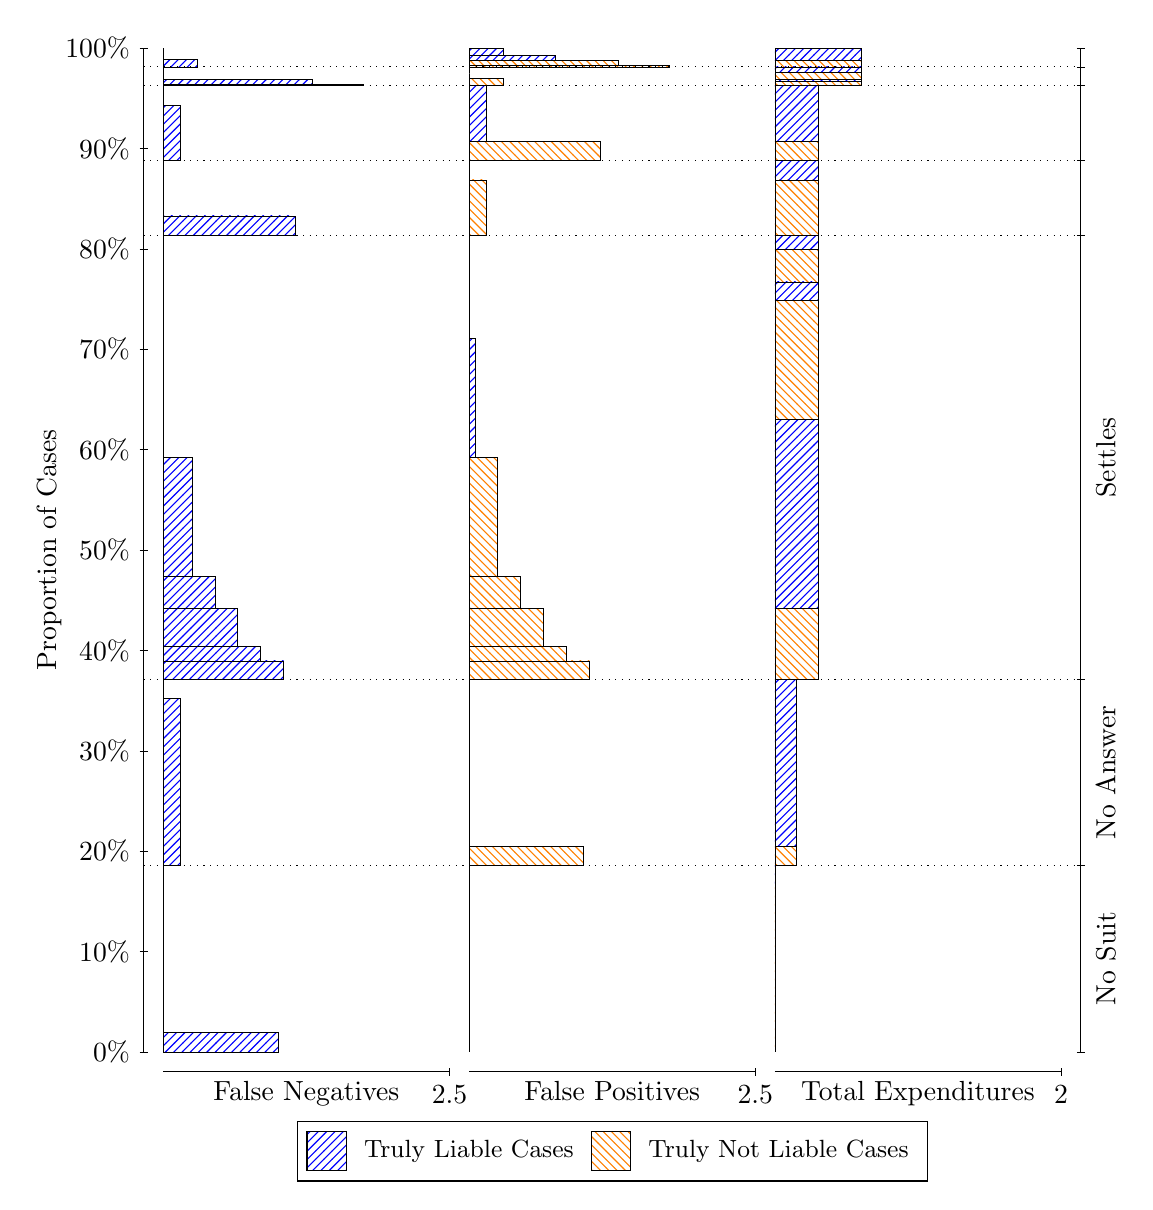
\begin{tikzpicture}
\draw[black, very thin] (1.5,1.75) -- (1.5,14.5);
\node[rotate=90, text=black, anchor=center] at (0.3, 8.125) {Proportion of Cases};
\draw[black, very thin] (1.45,1.75) -- (1.55,1.75);
\node[text=black, anchor=east] at (1.45, 1.75) {0\%};
\draw[black, very thin] (1.45,3.025) -- (1.55,3.025);
\node[text=black, anchor=east] at (1.45, 3.025) {10\%};
\draw[black, very thin] (1.45,4.3) -- (1.55,4.3);
\node[text=black, anchor=east] at (1.45, 4.3) {20\%};
\draw[black, very thin] (1.45,5.575) -- (1.55,5.575);
\node[text=black, anchor=east] at (1.45, 5.575) {30\%};
\draw[black, very thin] (1.45,6.85) -- (1.55,6.85);
\node[text=black, anchor=east] at (1.45, 6.85) {40\%};
\draw[black, very thin] (1.45,8.125) -- (1.55,8.125);
\node[text=black, anchor=east] at (1.45, 8.125) {50\%};
\draw[black, very thin] (1.45,9.4) -- (1.55,9.4);
\node[text=black, anchor=east] at (1.45, 9.4) {60\%};
\draw[black, very thin] (1.45,10.675) -- (1.55,10.675);
\node[text=black, anchor=east] at (1.45, 10.675) {70\%};
\draw[black, very thin] (1.45,11.95) -- (1.55,11.95);
\node[text=black, anchor=east] at (1.45, 11.95) {80\%};
\draw[black, very thin] (1.45,13.225) -- (1.55,13.225);
\node[text=black, anchor=east] at (1.45, 13.225) {90\%};
\draw[black, very thin] (1.45,14.5) -- (1.55,14.5);
\node[text=black, anchor=east] at (1.45, 14.5) {100\%};

\draw[black, very thin] (13.4,1.75) -- (13.4,14.5);
\draw[black, very thin] (13.35,1.75) -- (13.45,1.75);
\node[anchor=west] at (13.35, 1.75) {};
\draw[black, very thin] (13.35,4.1224) -- (13.45,4.1224);
\node[anchor=west] at (13.35, 4.1224) {};
\draw[black, very thin] (13.35,6.4775) -- (13.45,6.4775);
\node[anchor=west] at (13.35, 6.4775) {};
\draw[black, very thin] (13.35,12.123) -- (13.45,12.123);
\node[anchor=west] at (13.35, 12.123) {};
\draw[black, very thin] (13.35,13.072) -- (13.45,13.072);
\node[anchor=west] at (13.35, 13.072) {};
\draw[black, very thin] (13.35,14.022) -- (13.45,14.022);
\node[anchor=west] at (13.35, 14.022) {};
\draw[black, very thin] (13.35,14.261) -- (13.45,14.261);
\node[anchor=west] at (13.35, 14.261) {};
\draw[black, very thin] (13.35,14.5) -- (13.45,14.5);
\node[anchor=west] at (13.35, 14.5) {};

\draw[black, very thin, pattern color=blue, pattern=north east lines] (1.75,1.75) rectangle (3.2033,1.9996);
\draw[black, very thin, pattern color=orange, pattern=north west lines] (1.75,1.9996) rectangle (1.75,4.1224);
\draw[black, very thin, pattern color=blue, pattern=north east lines] (1.75,4.1224) rectangle (1.968,6.2365);
\draw[black, very thin, pattern color=orange, pattern=north west lines] (1.75,6.2365) rectangle (1.75,6.4775);
\draw[black, very thin, pattern color=blue, pattern=north east lines] (1.75,6.4775) rectangle (3.276,6.7163);
\draw[black, very thin, pattern color=blue, pattern=north east lines] (1.75,6.7163) rectangle (2.9853,6.9008);
\draw[black, very thin, pattern color=blue, pattern=north east lines] (1.75,6.9008) rectangle (2.6947,7.3834);
\draw[black, very thin, pattern color=blue, pattern=north east lines] (1.75,7.3834) rectangle (2.404,7.7907);
\draw[black, very thin, pattern color=blue, pattern=north east lines] (1.75,7.7907) rectangle (2.1133,9.3002);
\draw[black, very thin, pattern color=orange, pattern=north west lines] (1.75,9.3002) rectangle (1.75,12.123);
\draw[black, very thin, pattern color=blue, pattern=north east lines] (1.75,12.123) rectangle (3.4213,12.369);
\draw[black, very thin, pattern color=orange, pattern=north west lines] (1.75,12.369) rectangle (1.75,13.072);
\draw[black, very thin, pattern color=blue, pattern=north east lines] (1.75,13.072) rectangle (1.968,13.775);
\draw[black, very thin, pattern color=orange, pattern=north west lines] (1.75,13.775) rectangle (1.75,14.022);
\draw[black, very thin, pattern color=blue, pattern=north east lines] (1.75,14.022) rectangle (4.2933,14.041);
\draw[black, very thin, pattern color=blue, pattern=north east lines] (1.75,14.041) rectangle (3.6393,14.106);
\draw[black, very thin, pattern color=orange, pattern=north west lines] (1.75,14.106) rectangle (1.75,14.261);
\draw[black, very thin, pattern color=blue, pattern=north east lines] (1.75,14.261) rectangle (2.186,14.356);
\draw[black, very thin, pattern color=orange, pattern=north west lines] (1.75,14.356) rectangle (1.75,14.44);
\draw[black, very thin, pattern color=blue, pattern=north east lines] (1.75,14.44) rectangle (1.75,14.5);
\draw[black, very thin, pattern color=orange, pattern=north west lines] (5.6333,1.75) rectangle (5.6333,3.8728);
\draw[black, very thin, pattern color=blue, pattern=north east lines] (5.6333,3.8728) rectangle (5.6333,4.1224);
\draw[black, very thin, pattern color=orange, pattern=north west lines] (5.6333,4.1224) rectangle (7.0867,4.3634);
\draw[black, very thin, pattern color=blue, pattern=north east lines] (5.6333,4.3634) rectangle (5.6333,6.4775);
\draw[black, very thin, pattern color=orange, pattern=north west lines] (5.6333,6.4775) rectangle (7.1593,6.7163);
\draw[black, very thin, pattern color=orange, pattern=north west lines] (5.6333,6.7163) rectangle (6.8687,6.9008);
\draw[black, very thin, pattern color=orange, pattern=north west lines] (5.6333,6.9008) rectangle (6.578,7.3834);
\draw[black, very thin, pattern color=orange, pattern=north west lines] (5.6333,7.3834) rectangle (6.2873,7.7907);
\draw[black, very thin, pattern color=orange, pattern=north west lines] (5.6333,7.7907) rectangle (5.9967,9.3002);
\draw[black, very thin, pattern color=blue, pattern=north east lines] (5.6333,9.3002) rectangle (5.706,10.81);
\draw[black, very thin, pattern color=blue, pattern=north east lines] (5.6333,10.81) rectangle (5.6333,12.123);
\draw[black, very thin, pattern color=orange, pattern=north west lines] (5.6333,12.123) rectangle (5.8513,12.826);
\draw[black, very thin, pattern color=blue, pattern=north east lines] (5.6333,12.826) rectangle (5.6333,13.072);
\draw[black, very thin, pattern color=orange, pattern=north west lines] (5.6333,13.072) rectangle (7.3047,13.319);
\draw[black, very thin, pattern color=blue, pattern=north east lines] (5.6333,13.319) rectangle (5.8513,14.022);
\draw[black, very thin, pattern color=orange, pattern=north west lines] (5.6333,14.022) rectangle (6.0693,14.117);
\draw[black, very thin, pattern color=orange, pattern=north west lines] (5.6333,14.117) rectangle (5.6333,14.176);
\draw[black, very thin, pattern color=blue, pattern=north east lines] (5.6333,14.176) rectangle (5.6333,14.261);
\draw[black, very thin, pattern color=orange, pattern=north west lines] (5.6333,14.261) rectangle (8.1767,14.28);
\draw[black, very thin, pattern color=orange, pattern=north west lines] (5.6333,14.28) rectangle (7.5227,14.345);
\draw[black, very thin, pattern color=blue, pattern=north east lines] (5.6333,14.345) rectangle (6.7233,14.405);
\draw[black, very thin, pattern color=blue, pattern=north east lines] (5.6333,14.405) rectangle (6.0693,14.5);
\draw[black, very thin, pattern color=orange, pattern=north west lines] (9.5167,1.75) rectangle (9.5167,3.8728);
\draw[black, very thin, pattern color=blue, pattern=north east lines] (9.5167,3.8728) rectangle (9.5167,4.1224);
\draw[black, very thin, pattern color=orange, pattern=north west lines] (9.5167,4.1224) rectangle (9.7892,4.3634);
\draw[black, very thin, pattern color=blue, pattern=north east lines] (9.5167,4.3634) rectangle (9.7892,6.4775);
\draw[black, very thin, pattern color=orange, pattern=north west lines] (9.5167,6.4775) rectangle (10.062,7.3834);
\draw[black, very thin, pattern color=blue, pattern=north east lines] (9.5167,7.3834) rectangle (10.062,9.7828);
\draw[black, very thin, pattern color=orange, pattern=north west lines] (9.5167,9.7828) rectangle (10.062,11.292);
\draw[black, very thin, pattern color=blue, pattern=north east lines] (9.5167,11.292) rectangle (10.062,11.531);
\draw[black, very thin, pattern color=orange, pattern=north west lines] (9.5167,11.531) rectangle (10.062,11.938);
\draw[black, very thin, pattern color=blue, pattern=north east lines] (9.5167,11.938) rectangle (10.062,12.123);
\draw[black, very thin, pattern color=orange, pattern=north west lines] (9.5167,12.123) rectangle (10.062,12.826);
\draw[black, very thin, pattern color=blue, pattern=north east lines] (9.5167,12.826) rectangle (10.062,13.072);
\draw[black, very thin, pattern color=orange, pattern=north west lines] (9.5167,13.072) rectangle (10.062,13.319);
\draw[black, very thin, pattern color=blue, pattern=north east lines] (9.5167,13.319) rectangle (10.062,14.022);
\draw[black, very thin, pattern color=orange, pattern=north west lines] (9.5167,14.022) rectangle (10.607,14.081);
\draw[black, very thin, pattern color=blue, pattern=north east lines] (9.5167,14.081) rectangle (10.607,14.1);
\draw[black, very thin, pattern color=orange, pattern=north west lines] (9.5167,14.1) rectangle (10.607,14.195);
\draw[black, very thin, pattern color=blue, pattern=north east lines] (9.5167,14.195) rectangle (10.607,14.261);
\draw[black, very thin, pattern color=orange, pattern=north west lines] (9.5167,14.261) rectangle (10.607,14.345);
\draw[black, very thin, pattern color=blue, pattern=north east lines] (9.5167,14.345) rectangle (10.607,14.5);
\draw[black, dotted] (1.5,4.1224) -- (13.4,4.1224);
\draw[black, dotted] (1.5,6.4775) -- (13.4,6.4775);
\draw[black, dotted] (1.5,12.123) -- (13.4,12.123);
\draw[black, dotted] (1.5,13.072) -- (13.4,13.072);
\draw[black, dotted] (1.5,14.022) -- (13.4,14.022);
\draw[black, dotted] (1.5,14.261) -- (13.4,14.261);
\draw[black, very thin] (1.75,1.5) -- (5.3833,1.5);
\node[text=black, anchor=north] at (3.5667, 1.5) {False Negatives};
\draw[black, very thin] (5.3833,1.45) -- (5.3833,1.55);
\node[text=black, anchor=north] at (5.3833, 1.45) {2.5};

\draw[black, very thin] (5.6333,1.5) -- (9.2667,1.5);
\node[text=black, anchor=north] at (7.45, 1.5) {False Positives};
\draw[black, very thin] (9.2667,1.45) -- (9.2667,1.55);
\node[text=black, anchor=north] at (9.2667, 1.45) {2.5};

\draw[black, very thin] (9.5167,1.5) -- (13.15,1.5);
\node[text=black, anchor=north] at (11.333, 1.5) {Total Expenditures};
\draw[black, very thin] (13.15,1.45) -- (13.15,1.55);
\node[text=black, anchor=north] at (13.15, 1.45) {2};

\node[text=black, centered, rotate=90] at (13.72, 2.9362) {No Suit};
\node[text=black, centered, rotate=90] at (13.72, 5.2999) {No Answer};
\node[text=black, centered, rotate=90] at (13.72, 9.3002) {Settles};





\draw (7.449999999999999,1.5) node[draw=none] (baseCoordinate) {};
\begin{scope}[align=center]
        \matrix[scale=0.5, draw=black, below=0.5cm of baseCoordinate, nodes={draw}, column sep=0.1cm]{
            \node[rectangle, draw, minimum width=0.5cm, minimum height=0.5cm, pattern color=blue, pattern=north east lines] {}; &
            \node[draw=none, font=\small, text=black] (B) {Truly Liable Cases}; &
            \node[rectangle, draw, minimum width=0.5cm, minimum height=0.5cm, pattern color=orange, pattern=north west lines] {}; &
            \node[draw=none, font=\small, text=black] (B) {Truly Not Liable Cases}; \\
            };
\end{scope}

\end{tikzpicture}
\end{document}